\section{Überblick über den Optimierungsvorgang}
Die Ausführung des Programms geschieht in drei Schritten (vgl. Abb. \ref{Ablauf}): (1) Konfiguration, (2) Generierung von semantisch gleichen Plänen, (3) Finden des optimalen Plans.

\begin{figure}[h]
  \centering
  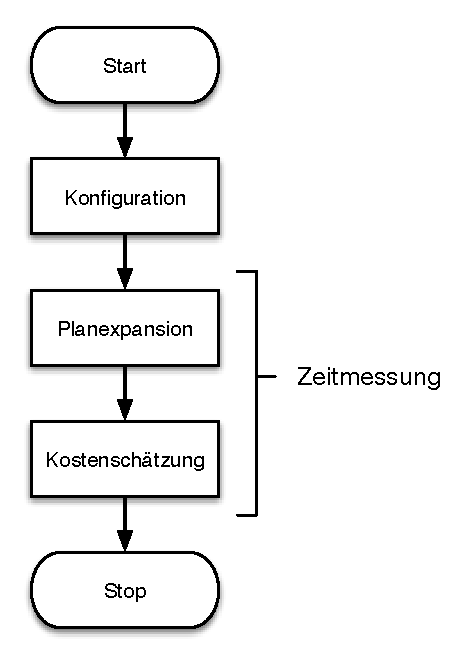
\includegraphics{04_Implementierung/Ablauf.pdf}
  \caption{Ablauf der eigenen Implementierung}
  \label{Ablauf}
\end{figure}


Im ersten Schritt, wird auf Grund von externen Parametern das System konfiguriert. Die Konfiguration erfolgt durch ein JSON File. In ihm werden die Parameter für die Optimierung festgelegt:

\begin{itemize}
\item Relationen und deren Kardinalität 
\item JoinEdges und deren Selektvität
\item Initial-Plan
\item Regelsets
\end{itemize}

Mit Hilfe der Relationen und deren Kardinalität können später im Zusammenspiel mit JoinEdges und Selektivitität die Kosten für einen Plan berechnet werden. Der initiale Plan dient als Startpunkt der Transformation. Auf ihn werden die Regelsets angewendet und so logische  Äquivalente erzeugt.

Zu Beginn des zweiten Schritts, der Erzeugung von äquivalenten Plänen, wird die Zeitmessung gestartet.  Mit Hilfe von Exektoren werden die unterschiedlichen Regelsets auf den Initialen Plan angewendet. Für jeden Knoten wird zuerst festgestellt, ob er bereits expanded wurde. Falls das nicht der Fall ist, wird geprüft, ob eine Regel aus dem Regelset anwendbar ist. iI

In einem finalen Schritt wird findet die Kostenberechnung statt und aus den möglichen Plänen wird der günstigste ausgewählt. Diese Preisberechnung findet im Modul der Kostenschätzung statt.


\section{Unterschiede zu Volcano und Pyro(J)}

Einer der fundamentalen Unterschiede zwischen Pyro bzw. Volcano zur hier vorgestellten Implementierung ist, dass sowohl Volcano als auch Pyro vollständige Optimierer sind. Sie erstellen basierend auf einer Anfrage einen physischen Plan, der dann weiterverarbeitet werden kann. Im Gegensatz dazu wird für diese Masterarbeit nur das Join-Ordering betrachtet und daher auch nur das Join-Ordering implementiert.


Ebenfalls wird von Volcano und Pyro immer ein physischer Plan erzeugt. Dies geschieht in dieser Implementierung nicht. Es werden somit nur für die logischen Pläne Alternativen gefunden und aus diesen Alternativen der günstigste Plan ausgewählt. Dies geschieht, da für die Überprüfung der Regelsets RS-B0, RS-B1, RS-B2 und GraphRule keine pysischen Pläne notwendig sind. Die unterschiedlichen Rulesets widmen sich nicht dem Berechnen von physischen Alternativen, sondern dem Finden alternativer Join-Reihenfolgen. Falls alle Pläne gefunden werden, wäre der Aufwand für die Umwandlung in physische Pläne für alle Rulesets gleich. Daher trägt die Umwandlung und weitere Expansion nicht zu Unterschieden in der Expansionsgeschwindigkeit bei.

Ein weiterer Unterschied zu Volcano ist, dass alle Pläne direkt berechnet werden und  anschließend aus allen Plänen der günstigste Plan ausgewählt wird. Volcano berechnet zuerst einen Plan und wählt dann aus der Menge der physischen Pläne den günstigsten aus, bevor der nächste logische Plan berechnet wird. Nur falls ein günstigerer Plan gefunden wird, wird dieser auch im Speicher behalten. Im Gegensatz zu diesem sehr ressourcensparenden Verfahren setzt Pyro und die eigen Implementierung auf Pläne die dauerhaft vorgehalten werden. Dies erleichtert das Debugging, da alle Pläne jederzeit betrachtet werden können, erhöht aber den Verbrauch an Arbeitsspeicher.

Neben diesen konzeptionellen Unterschieden setzt die implementierte Lösung wie Pyro oder Volcano auf C++ als Programmiersprache). Im Gegensatz zu diesen Implementierungen setzt PyroJ auf Java und die Java Plattform, die per se mit schlecht beeinflussbaren Faktoren wie Garbage Collection, Virtuellen Maschinen und JIT-Compilern zu kämpfen hat. Wie bereits in Kapitel \ref{} besprochen, mussten bei den Messungen mit PyroJ diverse Parameter gesetzt werden, um überhaupt reproduzierbare Ergebnisse zu erzeugen. Um solchen Problemen vorzubeugen, wurde vollständig auf C++ für die Implementierung gesetzt. Da der Code zur Laufzeit bereits vollständig kompiliert ist, können Probleme durch einen JIT Compiler und Optimierungen zur Laufzeit ausgeschlossen werden. Unterbrechungen durch eine Garbage Collection können nicht auftreten, da keine vorhanden sind.